\documentclass[]{book}
\usepackage{lmodern}
\usepackage{amssymb,amsmath}
\usepackage{ifxetex,ifluatex}
\usepackage{fixltx2e} % provides \textsubscript
\ifnum 0\ifxetex 1\fi\ifluatex 1\fi=0 % if pdftex
  \usepackage[T1]{fontenc}
  \usepackage[utf8]{inputenc}
\else % if luatex or xelatex
  \ifxetex
    \usepackage{mathspec}
  \else
    \usepackage{fontspec}
  \fi
  \defaultfontfeatures{Ligatures=TeX,Scale=MatchLowercase}
  \newcommand{\euro}{€}
\fi
% use upquote if available, for straight quotes in verbatim environments
\IfFileExists{upquote.sty}{\usepackage{upquote}}{}
% use microtype if available
\IfFileExists{microtype.sty}{%
\usepackage{microtype}
\UseMicrotypeSet[protrusion]{basicmath} % disable protrusion for tt fonts
}{}
\usepackage[margin=1in]{geometry}
\usepackage{hyperref}
\PassOptionsToPackage{usenames,dvipsnames}{color} % color is loaded by hyperref
\hypersetup{unicode=true,
            pdftitle={q-sb},
            pdfauthor={Verena Kasztantowicz},
            pdfborder={0 0 0},
            breaklinks=true}
\urlstyle{same}  % don't use monospace font for urls
\usepackage{natbib}
\bibliographystyle{apalike}
\usepackage{longtable,booktabs}
\usepackage{graphicx,grffile}
\makeatletter
\def\maxwidth{\ifdim\Gin@nat@width>\linewidth\linewidth\else\Gin@nat@width\fi}
\def\maxheight{\ifdim\Gin@nat@height>\textheight\textheight\else\Gin@nat@height\fi}
\makeatother
% Scale images if necessary, so that they will not overflow the page
% margins by default, and it is still possible to overwrite the defaults
% using explicit options in \includegraphics[width, height, ...]{}
\setkeys{Gin}{width=\maxwidth,height=\maxheight,keepaspectratio}
\setlength{\parindent}{0pt}
\setlength{\parskip}{6pt plus 2pt minus 1pt}
\setlength{\emergencystretch}{3em}  % prevent overfull lines
\providecommand{\tightlist}{%
  \setlength{\itemsep}{0pt}\setlength{\parskip}{0pt}}
\setcounter{secnumdepth}{5}

%%% Use protect on footnotes to avoid problems with footnotes in titles
\let\rmarkdownfootnote\footnote%
\def\footnote{\protect\rmarkdownfootnote}

%%% Change title format to be more compact
\usepackage{titling}

% Create subtitle command for use in maketitle
\newcommand{\subtitle}[1]{
  \posttitle{
    \begin{center}\large#1\end{center}
    }
}

\setlength{\droptitle}{-2em}
  \title{q-sb}
  \pretitle{\vspace{\droptitle}\centering\huge}
  \posttitle{\par}
  \author{Verena Kasztantowicz}
  \preauthor{\centering\large\emph}
  \postauthor{\par}
  \predate{\centering\large\emph}
  \postdate{\par}
  \date{2017-02-05}


% Redefines (sub)paragraphs to behave more like sections
\ifx\paragraph\undefined\else
\let\oldparagraph\paragraph
\renewcommand{\paragraph}[1]{\oldparagraph{#1}\mbox{}}
\fi
\ifx\subparagraph\undefined\else
\let\oldsubparagraph\subparagraph
\renewcommand{\subparagraph}[1]{\oldsubparagraph{#1}\mbox{}}
\fi

\usepackage{booktabs}

\begin{document}
\maketitle

{
\setcounter{tocdepth}{1}
\tableofcontents
}
\chapter{Einführung}\label{einfuhrung}

q-sb ist ein Seminarprojekt mit Grundschulpädagogik/Deutsch-Studierenden
der HU Berlin im Wintersemester 2016/2017. Die Frage ist: Wie soll
Sprachbetrachtung, als zentraler Arbeitsbereich der Deutschdidaktik,
gestaltet werden? Welche Präferenzen haben Studierende, Lehrer, Eltern,
Schüler und Personengruppen, die sich nicht tagtäglich mit didaktischen
Fragen befassen? Auf Grundlage der theoretischen Ansätze des Seminars
wurde gemeinsam ein Umfrageinstrument (Q-Methodologie) entwickelt und
mit 95 Teilnehmenden erprobt.

\chapter{Analyse}\label{analyse}

\section{Faktorerhaltung}\label{faktorerhaltung}

\section{Faktorexktration}\label{faktorexktration}

\begin{verbatim}
## Q-method analysis.
## Finished on:             Sun Feb  5 21:23:20 2017
## Original data:           37 statements, 91 Q-sorts
## Forced distribution:     FALSE
## Number of factors:       2
## Rotation:                varimax
## Flagging:                automatic
## Correlation coefficient: spearman
\end{verbatim}

\begin{figure}[htbp]
\centering
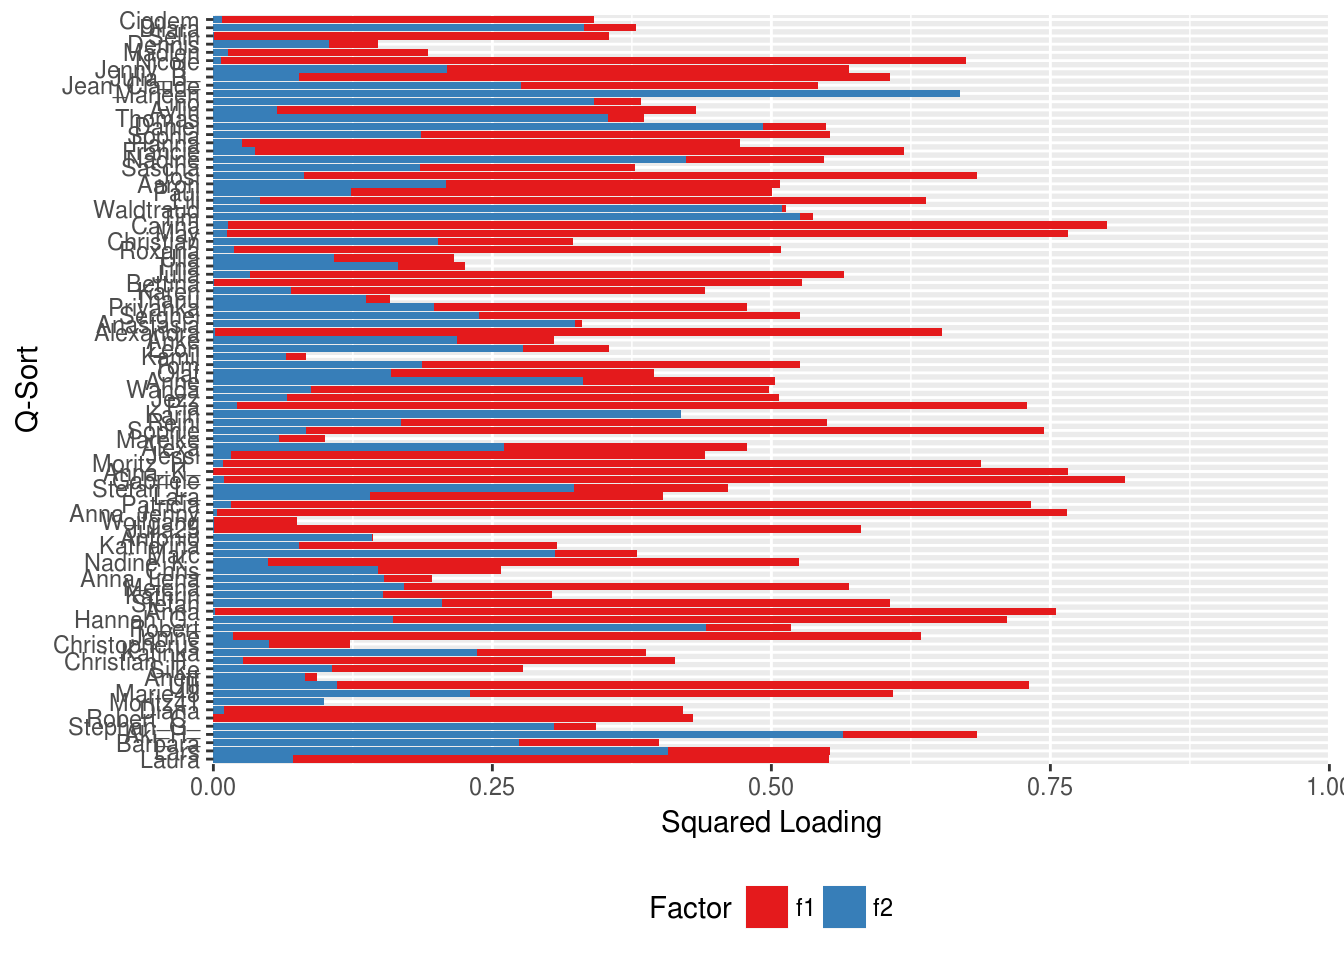
\includegraphics{Sprachbetrachtung_files/figure-latex/loas-comp-1.pdf}
\caption{\label{fig:loas-comp}Ladungen der Faktoren auf den Leute-Variablen}
\end{figure}

\begin{figure}[htbp]
\centering
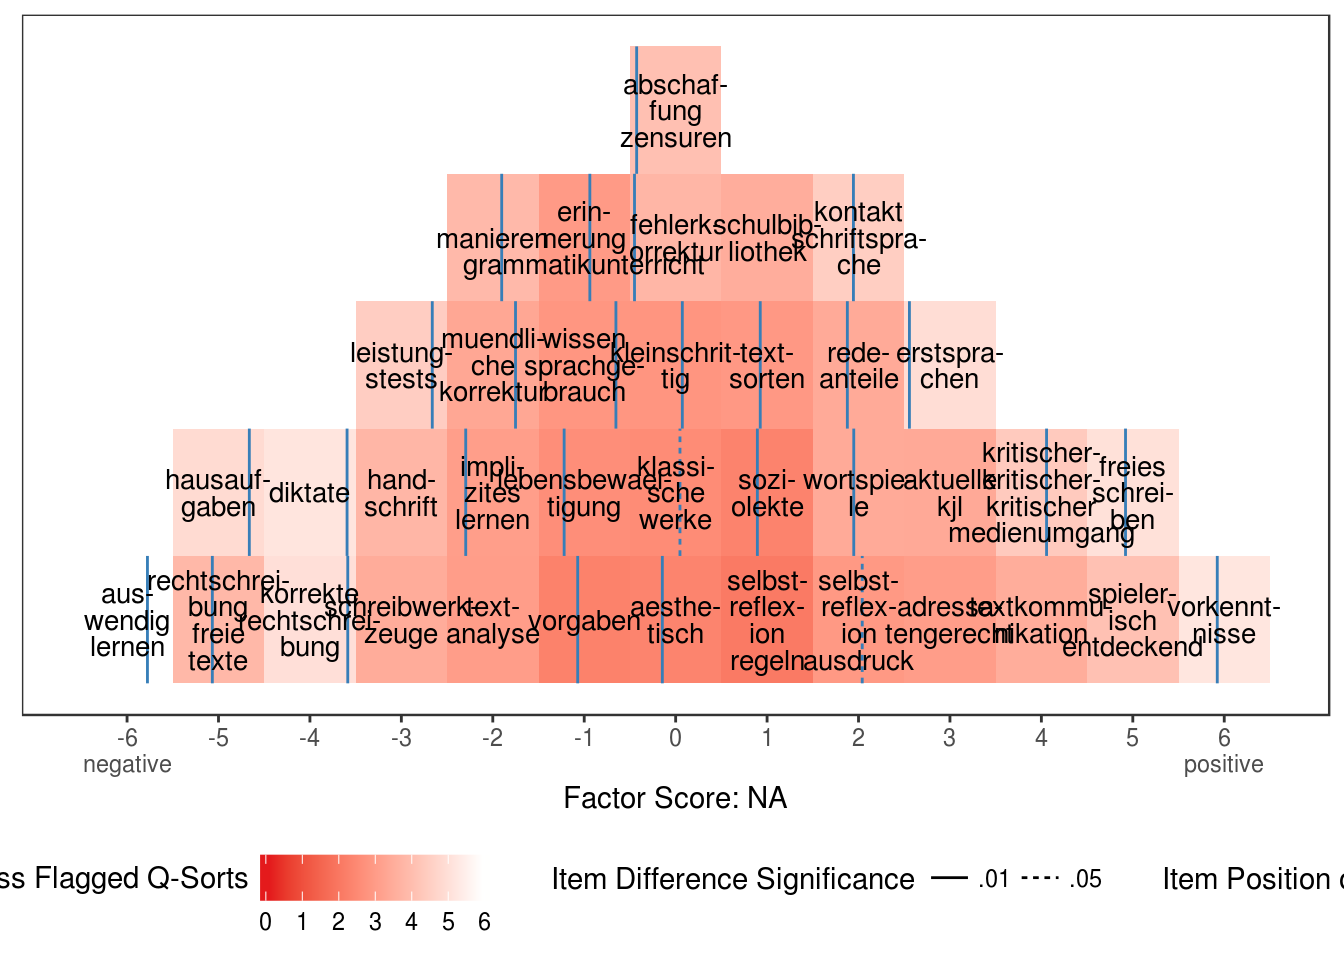
\includegraphics{Sprachbetrachtung_files/figure-latex/f1-1.pdf}
\caption{\label{fig:f1}Idealtypische Sortierungen Faktor 1}
\end{figure}

\begin{figure}[htbp]
\centering
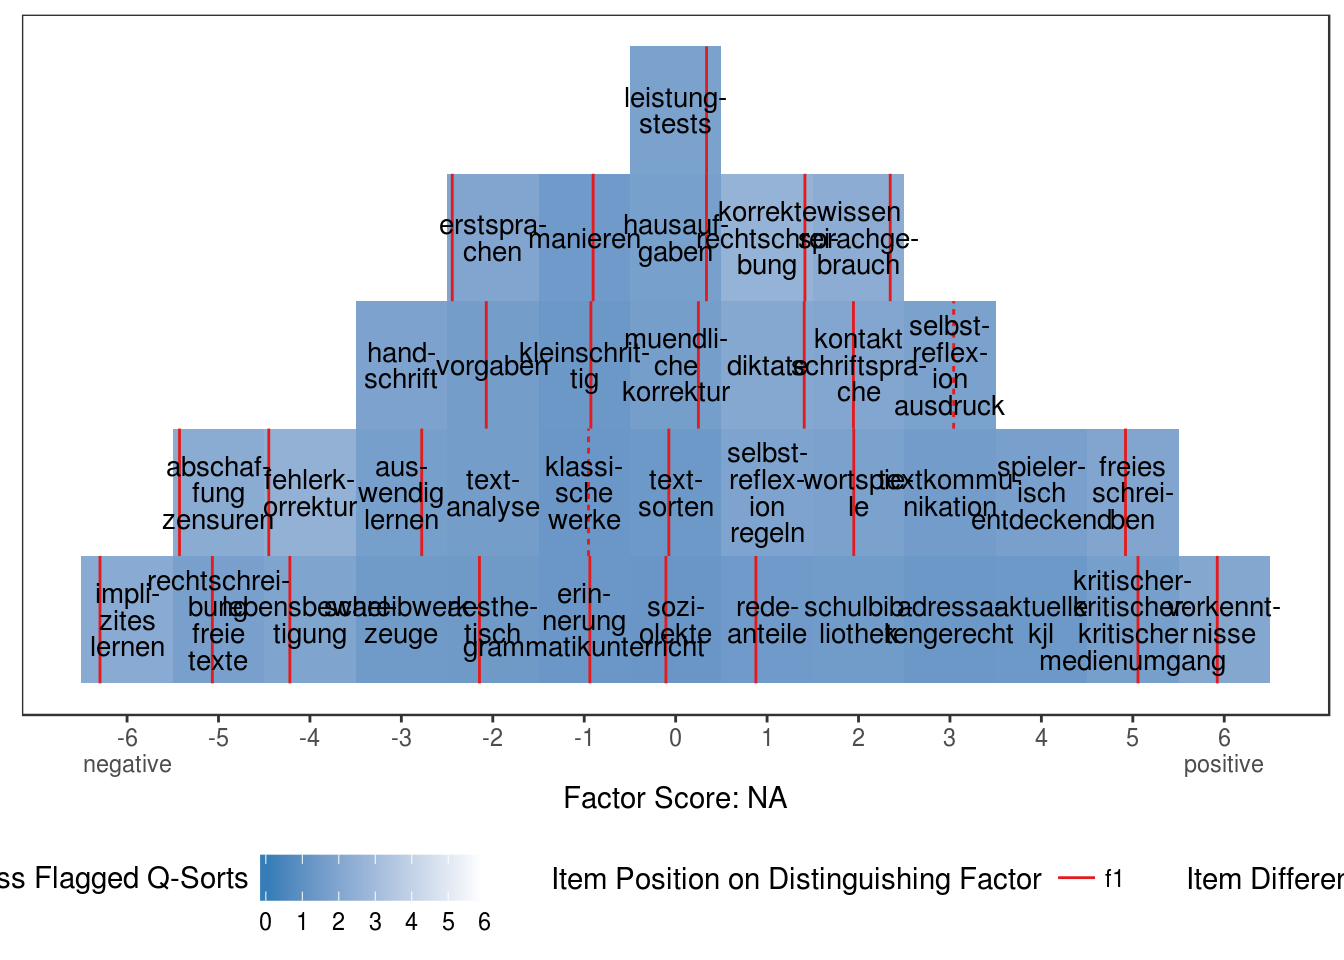
\includegraphics{Sprachbetrachtung_files/figure-latex/f2-1.pdf}
\caption{\label{fig:f2}Idealtypische Sortierungen Faktor 2}
\end{figure}

\end{document}
